\section{Технологический раздел}

\subsection{Выбор языка и библиотеки для разработки средства сбора данных}

В качестве средства реализации была выбрана библиотека Telebot, так как:

\begin{enumerate}
	\item[1.] Функционал приложения не предусматривает сложных операций, в силу чего низкая производительность ЯП Python не скажется на скорости отклика системы;
	\item[2.] ЯП Python позволит в короткий срок реализовать и отладить программный продукт;
	\item[3.] ЯП Python позволит быстро разворачивать приложение на разнообразных операционных системах, поддерживающих интерпретатор Python;
	\item[4.] Telebot предоставляет более тонкую настройку и контроль над запросами и ответами API Telegram.
\end{enumerate}

\subsection{Выбор СУБД}

% Для организации хранения данных будет задействована реляционная СУБД PostgreSQL \cite{postgres}. Выбор обусловлен постановкой задачи, не требующий со стороны базы данных дополнительных возможностей, а также высокой эффективности форматов хранения данных. Таким образом, данная СУБД сможет удовлетворить все потребности для решении задачи.
В задаче не определены никакие специальные возможности вспомогательного программного обеспечения для хранения данных. Таким образом, для эффективности работы с ними предполагается хранение классов локально в таблице формата CSV \cite{csv} с хранением резервной копии на удаленном сервере.

\subsection{Интерфейс средства сбора данных}

На рисунках \ref{img:teleg1}-\ref{img:teleg4} представлен интерфейс реализованного Telegram-бота.

\begin{figure}[H]
	\centering
	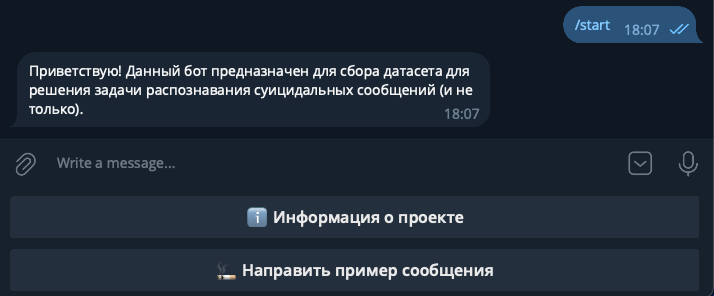
\includegraphics[width=\textwidth]{inc/teleg1.png}
	\caption{ Приветственное сообщение новому пользователю. }
	\label{img:teleg1}
\end{figure}

\begin{figure}[H]
	\centering
	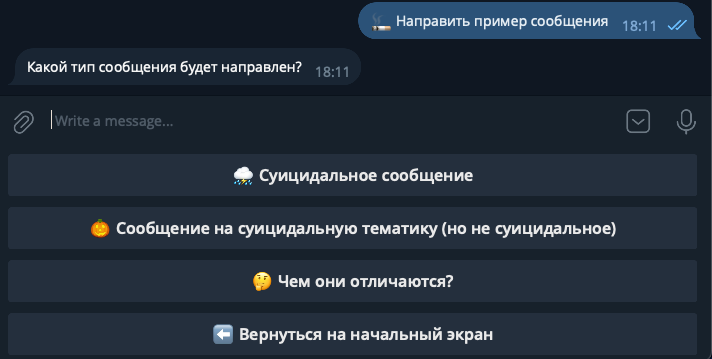
\includegraphics[width=\textwidth]{inc/teleg2.png}
	\caption{ Функционал направления в систему сообщения пользователем. }
	\label{img:teleg2}
\end{figure}

\begin{figure}[H]
	\centering
	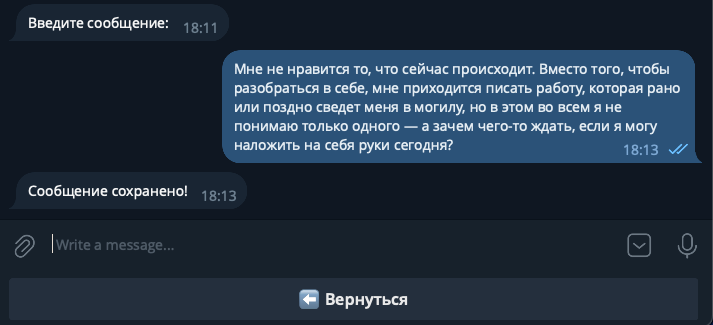
\includegraphics[width=\textwidth]{inc/teleg3.png}
	\caption{ Пример результата направленного в систему суицидального сообщения. }
	\label{img:teleg3}
\end{figure}

\begin{figure}[H]
	\centering
	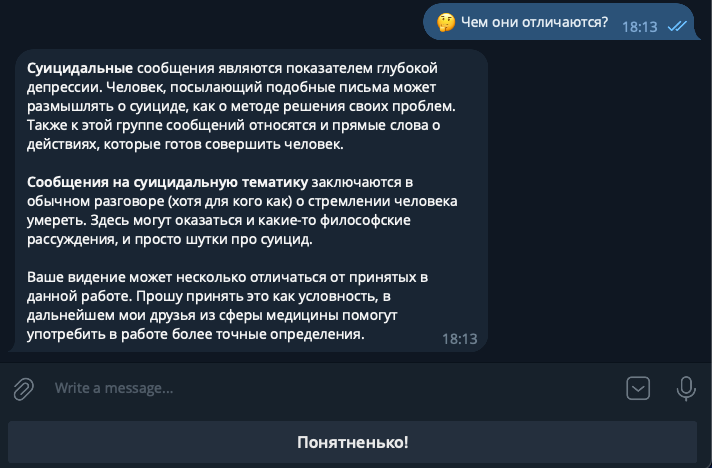
\includegraphics[width=\textwidth]{inc/teleg4.png}
	\caption{ Описание отличий суицидального сообщения и сообщения на суицидальную тематику. }
	\label{img:teleg4}
\end{figure}

\subsection{Описание обрабатываемых данных}

В результате работы средства сбора данных было размечено 1000 суицидальных сообщений. К собранным сообщениям было добавлено еще 1000 несуицидальных сообщений из датасета обнаружения пресуицидальных сигналов \cite{dataset}. 

На рисунке \ref{img:cloud1} представлена визуализация собранных данных класса суицидальных сообщений. Из представленного облака слов видно, что чаще всего в суицидальных сообщениях фигурирует слова ``жизнь'', ``мочь'' и ``хотеть''. Также стоит обратить внимание на присутствие слов ``суицид'', ``страдать'', ``депрессия'', ``смерть'', ``умирать'' и ``ад''.

\begin{figure}[H]
	\centering
	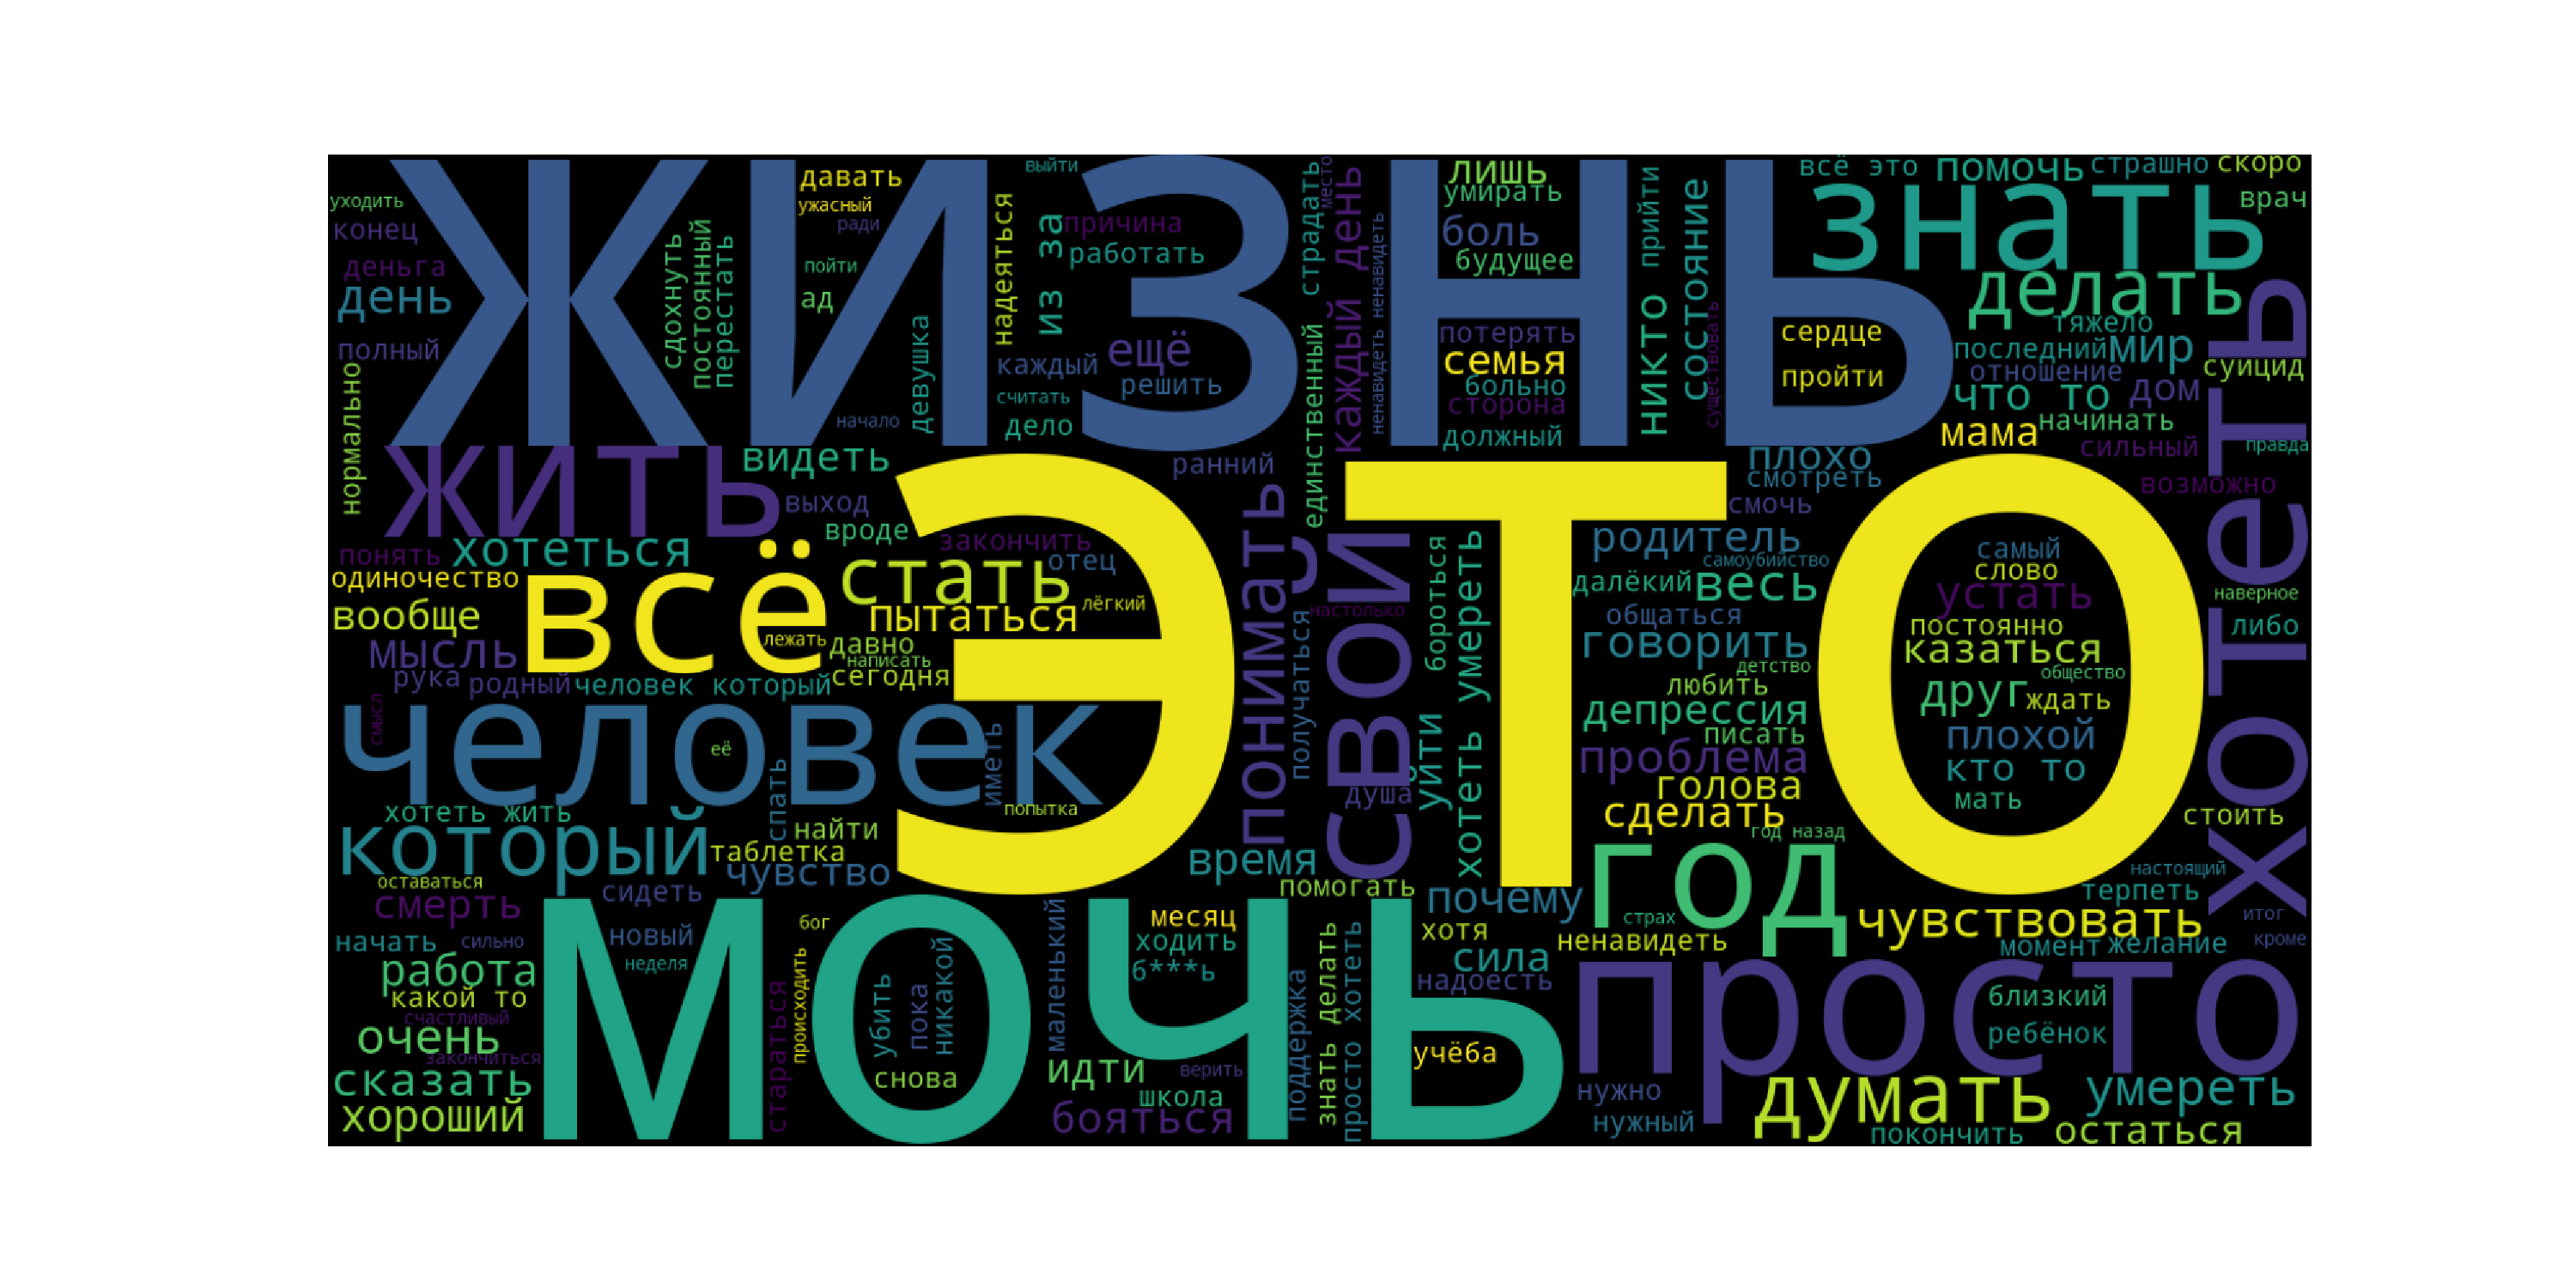
\includegraphics[width=\textwidth]{inc/cloudSuicidal.pdf}
	\caption{ Облако слов класса суицидальных сообщений. }
	\label{img:cloud1}
\end{figure}

На рисунке \ref{img:cloud2} представлена визуализация данных класса несуицидальных сообщений. Из представленного облака слов видно, что чаще всего в несуицидальных сообщениях встречаются слова ``хотеть'', ``человек'', а кроме того сообщения данной тематики чаще включают в себя различные вариации нецензурной брани.

\begin{figure}[H]
	\centering
	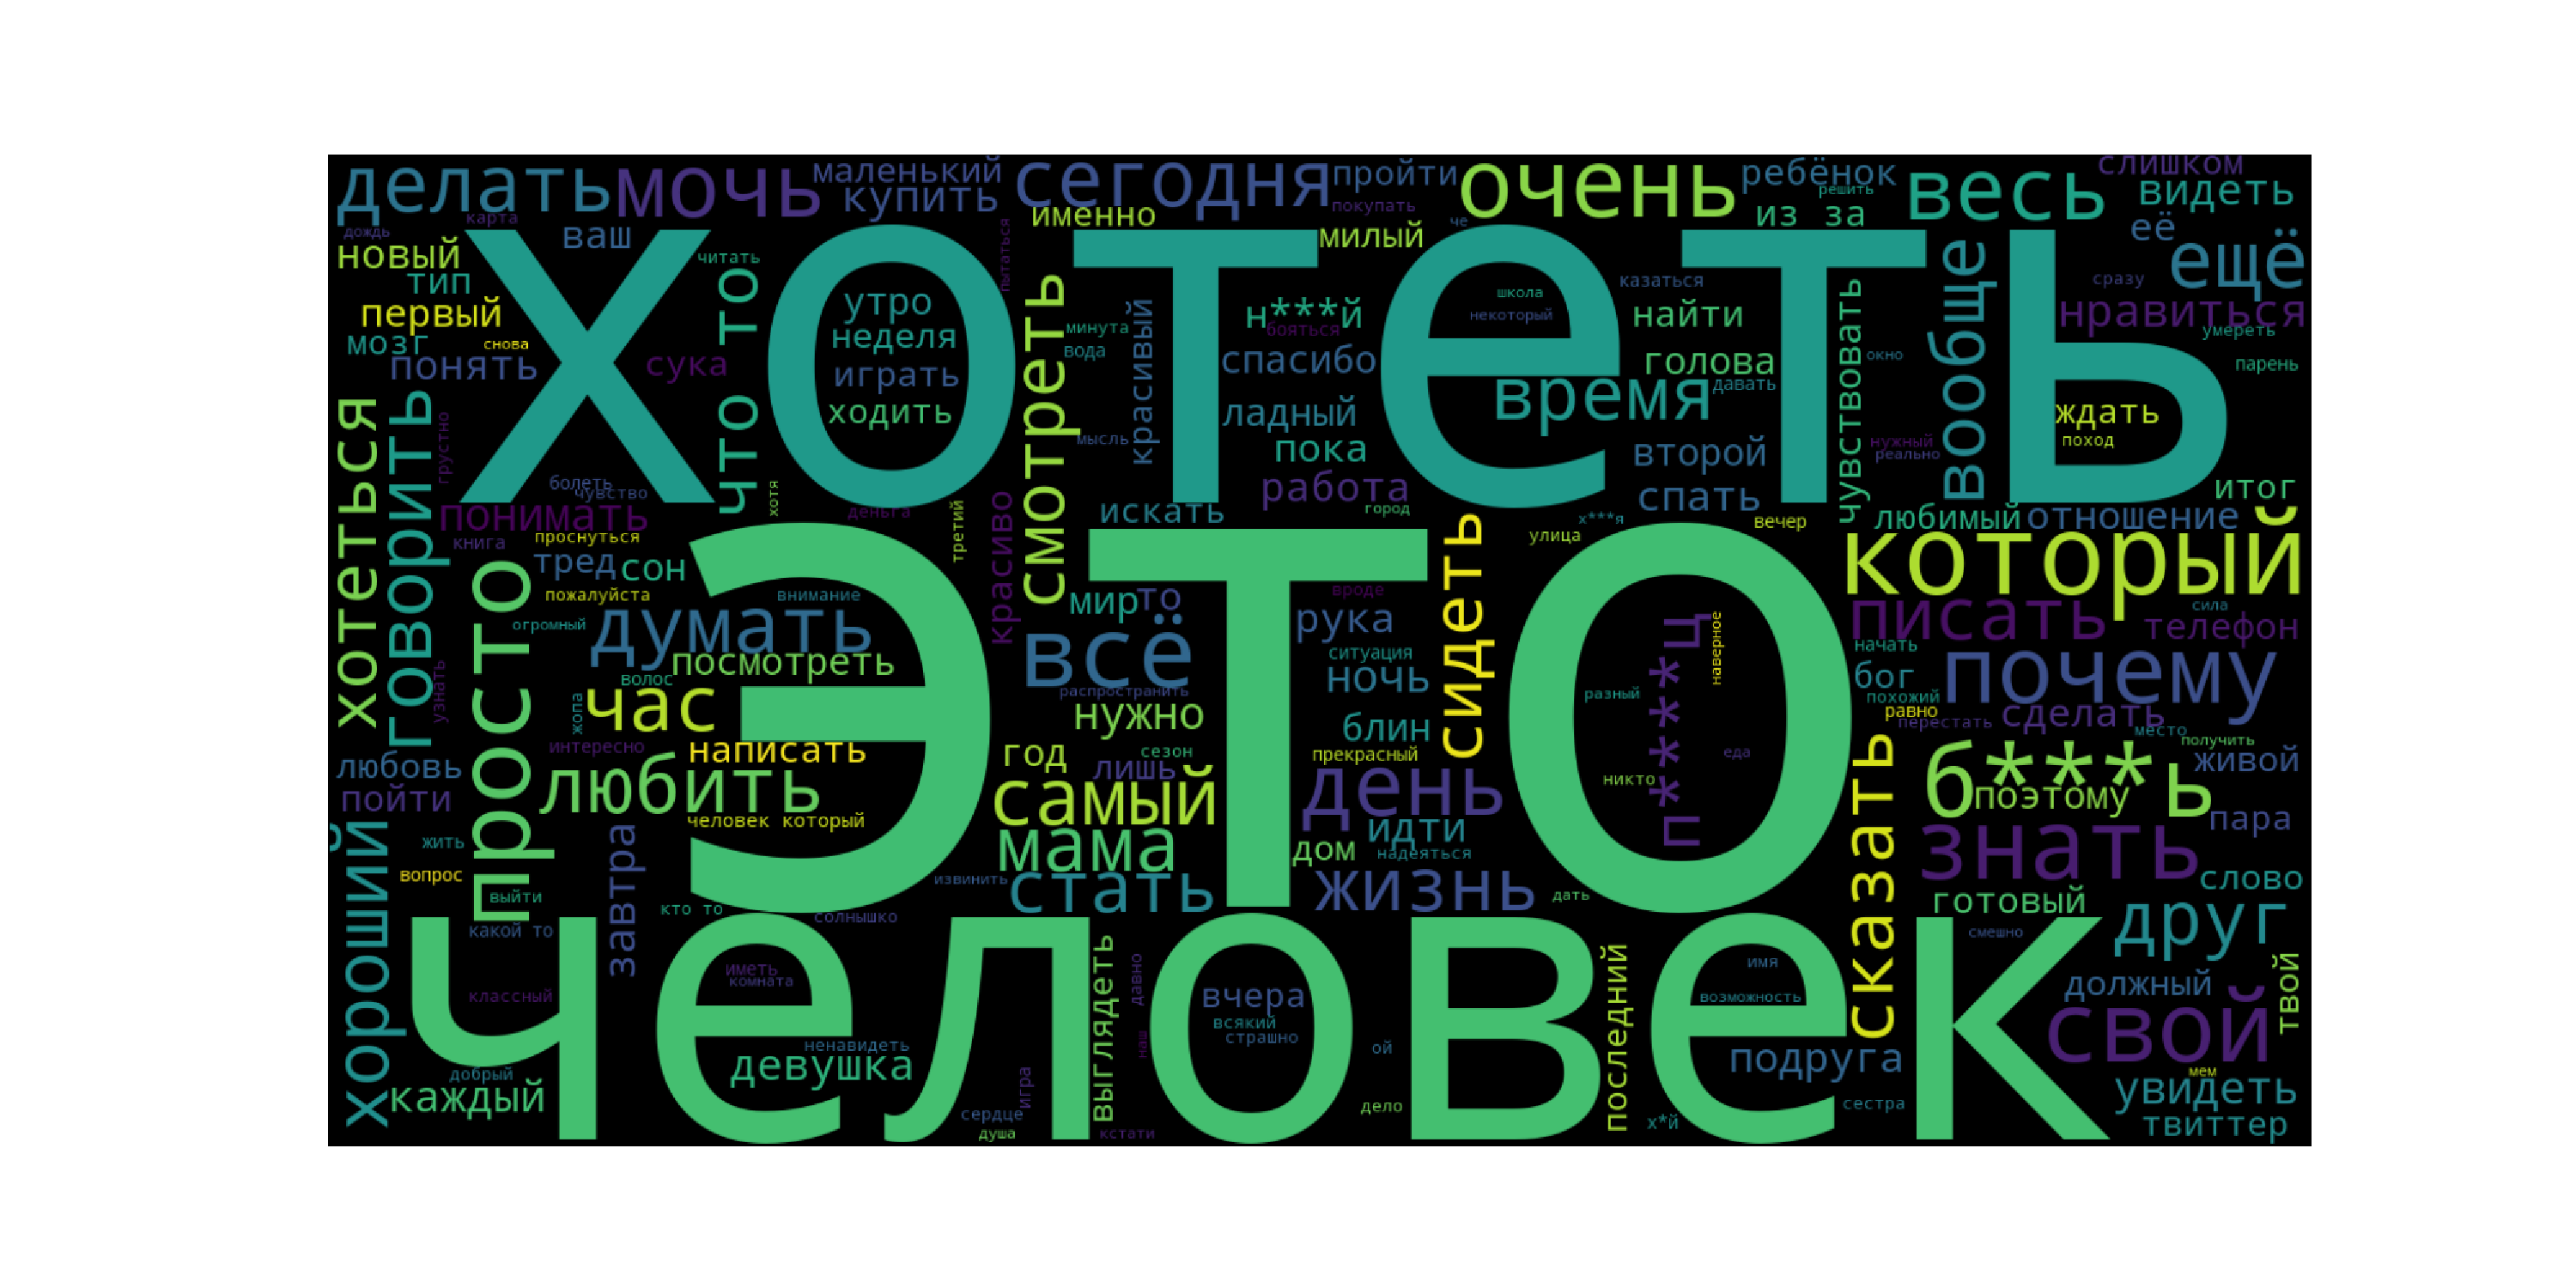
\includegraphics[width=\textwidth]{inc/cloudNonSuicidal.pdf}
	\caption{ Облако слов класса несуицидальных сообщений. }
	\label{img:cloud2}
\end{figure}

Представленная информация подтверждает факт того, что выбранные классы разделимы и отличны частотой употребления как слов, так и тематик.

\subsection{Выбор языка и библиотеки для разработки метода распознавания суицидальных паттернов поведения человека по текстовым сообщениям}

\subsection{Интерфейс средства распознавания суицидальных паттернов поведения человека по текстовым сообщениям}

\subsection*{Вывод}

лалала-бла-бла-бла, wololo

В качестве средства реализации была выбрана библиотека Telebot. Продемонстрирован функционал реализованного бота в мессенджере Telegram.